\documentclass[11 pt]{article}
\usepackage[bmargin=1in,tmargin=1in,lmargin=1in,rmargin=1in]{geometry}
\usepackage[dvipsnames]{xcolor}
\usepackage{amsfonts,amsmath,amsthm,color,amssymb, url, enumerate, bbm}
\usepackage{pgfplotstable, pgfplots}
\usepackage{graphicx}
\usepackage{tikz}
\usetikzlibrary{patterns, arrows}
\usepackage{subcaption}
\usepackage[noend]{algpseudocode}
\usepackage{algorithm}
\usepackage{float}
\usepackage{hyperref}
\usepackage{wrapfig}
\hypersetup{
    colorlinks=true,
    linkcolor=blue,
    filecolor=magenta,      
    urlcolor=blue,
}
\newcommand*\GnuplotDefs{
        set samples 100;
        Binv(p,q)=exp(lgamma(p+q)-lgamma(p)-lgamma(q));
        beta(x,p,q)=p<=0||q<=0?1/0:x<0||x>1?0.0:Binv(p,q)*x**(p-1.0)*(1.0-x)**(q-1.0);
    }

\title{Hotel Simulation Walk-through}
\author{Henry Robbins
\thanks{(hwr26@cornell.edu) Undergraduate Engineering School, Cornell University, Ithaca, New York, 14850.}}
\date{}

\begin{document}

\maketitle

\section{Introduction}

\par In this walk-through, we introduce a tool to help hotels make room assignment and housekeeping scheduling decisions. Here, we focus on hotel room assignment. In practice, hotel room assignments are often made through a combination of heuristics. For example, some front desk agents will assign ``higher quality" rooms first. However, in many cases, these heuristics do not provide the ``best" room assignment. This tool provides a variety of solvers (including in-practice heuristics) that a hotel can use to generate ideal room assignments. Furthermore, this tool allows hotels to assess their current assignment practices against ideal practices for both real and simulated instances.
\par The walk-through is organized as follows. Section 2 describes the room assignment problem and the information our tool uses to solve it. Furthermore, we introduce a sample instance which serves as a running example for the remainder of the walk-through. Section 3 provides a brief introduction to AMPL, its capabilities, and the necessary setup. Lastly, Sections 4 and 5 walk through the functionality of the tool at two different levels of expertise. Section 4 is aimed towards a front desk agent who may have no programming experience. Alternatively, Section 5 is aimed towards readers with a more technical background. It assumes some experience in Java (experience in AMPL is also helpful but not necessary). Furthermore, both assume the user is comfortable creating and manipulating CSV files in Excel or another spreadsheet software. 

\section{Problem Instance and Running Example}

\par First, we formally define the room assignment problem. There are a number of inputs that go into making a hotel room assignment. The relevant inputs this tool uses are listed below.
\begin{itemize}
    \item The set of rooms available to incoming guests
    \begin{itemize}
        \item The room number for each room
        \item The room type of each room (1 = Single, 2 = Double, 3 = Suite, etc.)
        \item The quality of each room (average satisfaction a guest has with the room)
    \end{itemize}
    \item The set of incoming guests
    \begin{itemize}
        \item An ID for each guest
        \item The room type each guest is requesting
        \item The time at which each guest arrives 
    \end{itemize}
    \item The satisfaction each guest has with each of the available rooms
\end{itemize}
\par This tool makes a few assumptions about these inputs. First, we assume there is no overbooking. Thus, there exists a room assignment where all guests are accommodated. Next, a guest's satisfaction is measured between 0 and 1 corresponding to between 0 and 100\% satisfied. Lastly, room types are ordered such that a greater type can accommodate all requests for its type and lower. E.g. type 1 might correspond to a Single and type 2 might correspond to a Double. A guest requesting type 1 can be assigned to type 2 but not vice versa.
\par These problem inputs (which we call an instance) can be represented with a set of CSV files. First, we have a CSV file representing the hotel. This file contains a row for each room. The first two columns describe the room number and type. The last column denotes the quality of the room. Room quality can be viewed as the satisfaction the average guest would have if assigned to this room. Below, are the relevant columns of \texttt{hotel.csv}, the CSV file representing the hotel in our running example. Room number 3 is of type 1. The average guest will have a satisfaction of 70\% if assigned this room.
\begin{center}
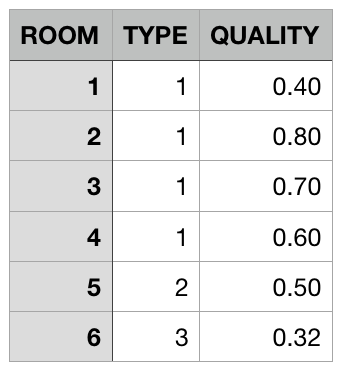
\includegraphics[scale=0.7]{images/roomsCSV.png}
\end{center}
\par Next, we have a CSV file representing the set of arrivals. This file contains a row for each arrival/guest. Similar to the hotel CSV, the first two columns denote a guest ID and the room type the guest is requesting. The last column denotes the arrival time of the guest in time intervals. In our running example, each time interval corresponds to 30 minutes. Below, is \texttt{arrivals.csv}, the CSV file representing the set of arrivals in our running example. Guest 4 is requesting room type 2 and arrives at time interval 34 equivalent to 1,020 minutes (since midnight) or 5PM. 
\begin{center}
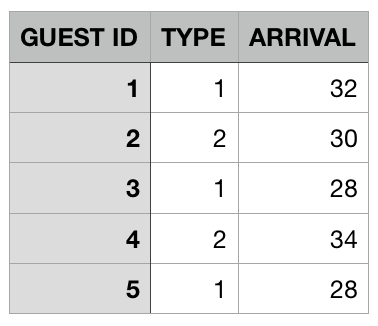
\includegraphics[scale=0.7]{images/arrivalsCSV.png}
\end{center}
\par Lastly, we have a CSV file representing the satisfaction each guest has with each room. Each row of this file corresponds to a guest while each column corresponds to a hotel room. The entry at each guest, room pair denotes the satisfaction that guest will have if placed in that room. Below, is \texttt{weights.csv}, the CSV file representing the guest satisfaction in our running example. Guest 2 has a satisfaction of 0\% with rooms 1-4. This is because guest 2 requests type 2 and rooms 1-4 are of type 1. Hence, guest 2 can not be feasibly assigned to any of these rooms so the satisfaction is 0. Furthermore, guest 2 has satisfaction of 50\% with both rooms 5 and 6. In this example, there is a lot of disagreement between guests. While guest 5 is 100\% satisfied with room 1, guest 3 is 20\% satisfied. Why might this be? One possible explanation is that room 1 is on the first floor. Guest 5 has mobility issues and really prefers first floor rooms. Meanwhile, guest 3 wants a great view and prefers rooms on higher floors. A hotel may have this knowledge from guests' previous visits and use it to estimate their satisfaction.
\begin{center}
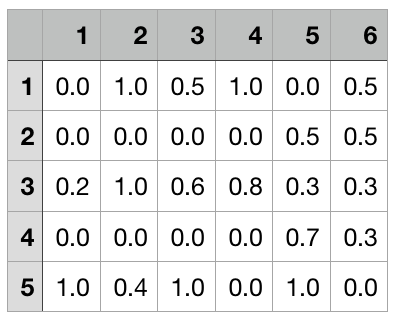
\includegraphics[scale=0.7]{images/weightsCSV.png}
\end{center}

\par Given these inputs, our tool outputs an assignment of guests to hotel rooms. For a room assignment to be feasible, each guest must be assigned to exactly one of the available rooms. Similarly, no room is assigned to more than one guest. Note that a guest will be assigned to one room but may represent multiple people who will share the room. Lastly, a guest is always assigned to a room of their requested type or upgraded to a higher type. There may be many feasible room assignments. Often, the goal is to choose the one with the highest guest satisfaction. Below, are two feasible room assignments.
\begin{center}
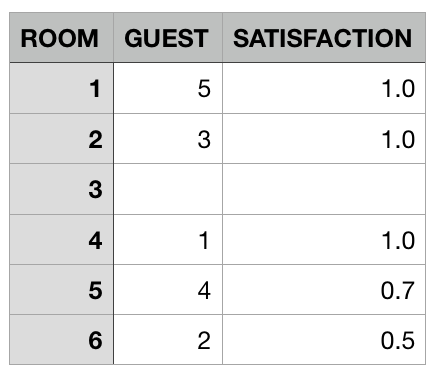
\includegraphics[scale=0.6]{images/optMeanAssign.png} \qquad
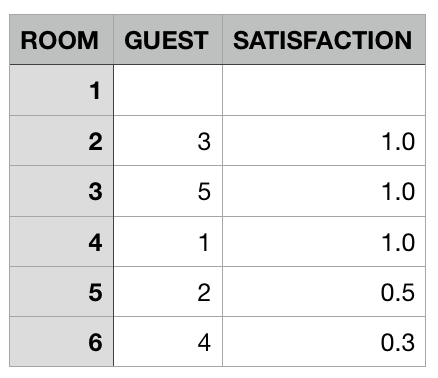
\includegraphics[scale=0.6]{images/bestAssign.png}
\end{center}
\par The assignment on the left yields a mean guest satisfaction of 84\%. Furthermore, the least satisfied guest (guest 2) is still 50\% satisfied. Alternatively, the assignment on the right has a mean guest satisfaction of 76\% and the least satisfied guest (guest 4) is only 30\% satisfied. Between these two assignments, it stands to reason we would select the left.

\newpage

\section{AMPL Setup}

AMPL is a powerful optimization software which implements many solvers for integer linear programming (ILP). We won't discuss ILPs further here. All that is needed to know is ILPs are an excellent way to formulate and solve a wide array of optimization problems including assignment, scheduling, transportation networks, etc. If you are interested in learning more, AMPL has a freely available book: \href{https://ampl.com/resources/the-ampl-book/}{AMPL: A Modeling Language
for Mathematical Programming}. This tool transforms hotel room assignent and scheduling problems into ILPs, uses AMPL's Java API to solve them, and then converts the ILP solution beck to a room assignment or schedule. In order to run most of the solvers this tool has to offer, the AMPL software must be downloaded. There is a free \href{https://ampl.com/try-ampl/download-a-free-demo/}{demo version} which will suffice for this walk-through. The demo version limits the size of the ILPs one can solve. The limit roughly translates to a maximum hotel size of 20. After downloading some version of AMPL, you will have a folder containing multiple files, including:
\begin{center}
    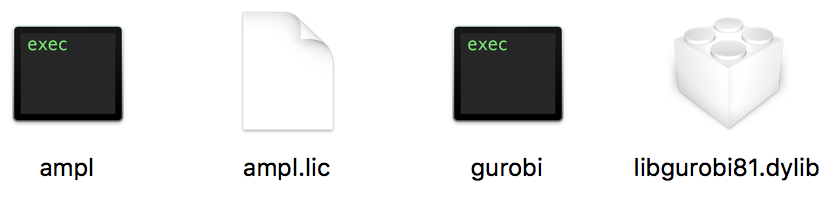
\includegraphics[scale=0.7]{images/amplFiles.png}
\end{center}
Lastly, the location of the AMPL folder must be specified. For the walk-through in Section 4 (no programming experience), the start screen will prompt you to specify the location of the AMPL folder. This is the folder containing the above files.
\begin{center}
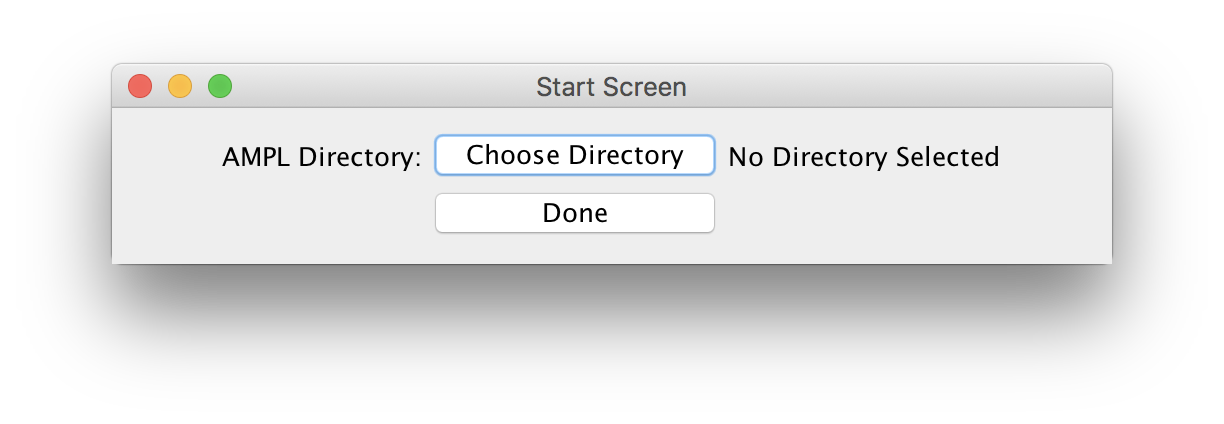
\includegraphics[scale=0.5]{images/startScreen.png}
\end{center}
 That completes the setup needed in Section 4. For the walk-through in Section 5 (some programming experience), the location is specified with the following line of code where ``/Users/Name/AMPL" will be replaced with the path to your AMPL folder.
 \begin{center}
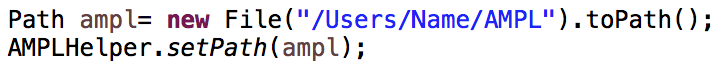
\includegraphics[scale=0.7]{images/codeAMPLsetup.png}
\end{center}
That concludes the setup required for AMPL. 

\section{No Programming Walk-through}
\par Upon opening the program, you are prompted to specify the location of the AMPL folder. After doing so, the simulation window of the application will appear. 
\newpage

\subsection{The Simulation Window}
Here, we give a brief description of each item on the simulation window.
\begin{enumerate}
    \item \textbf{Simulation Type:} This drop down menu allows the user to select which type of simulation they wish to run. The default simulation is called \texttt{Instance - Compare}. It allows for the comparison of different room assignment solvers on a specific instance.
    \item \textbf{Result Directory:} The results from each simulation are stored as a CSV file. Here, the user selects the location where that file should be placed.
    \item \textbf{Result File Name:} Here, the user provides the name of the resulting CSV file.
    \item \textbf{CSV File Inputs:} The simulation type \texttt{Instance - Compare} will run solvers on a specific instance. Recall, an instance is comprised of three CSV files which define it. Here, the user selects the hotel, arrivals, and weights CSV files respectively.
    \item \textbf{Solvers:} A solver represents an algorithm for producing a room assignment. They are discussed in more detail later in this section. The user can toggle which solvers should be run on the provided instance. Note: some of these solvers have parameters which can be set explicitly. Here, all solvers of this type are set to default values.
    \item \textbf{Statistics:} A statistic is some measure (such as mean guest satisfaction) on a room assignment (also discussed in more detail later). The user can toggle which statistics they would like computed on the assignment produced by every selected solver.
    \item \textbf{Run Simulation:} This button runs the simulation and the bar below shows the progress of the currently running simulation (if any).
\end{enumerate}
\begin{center}
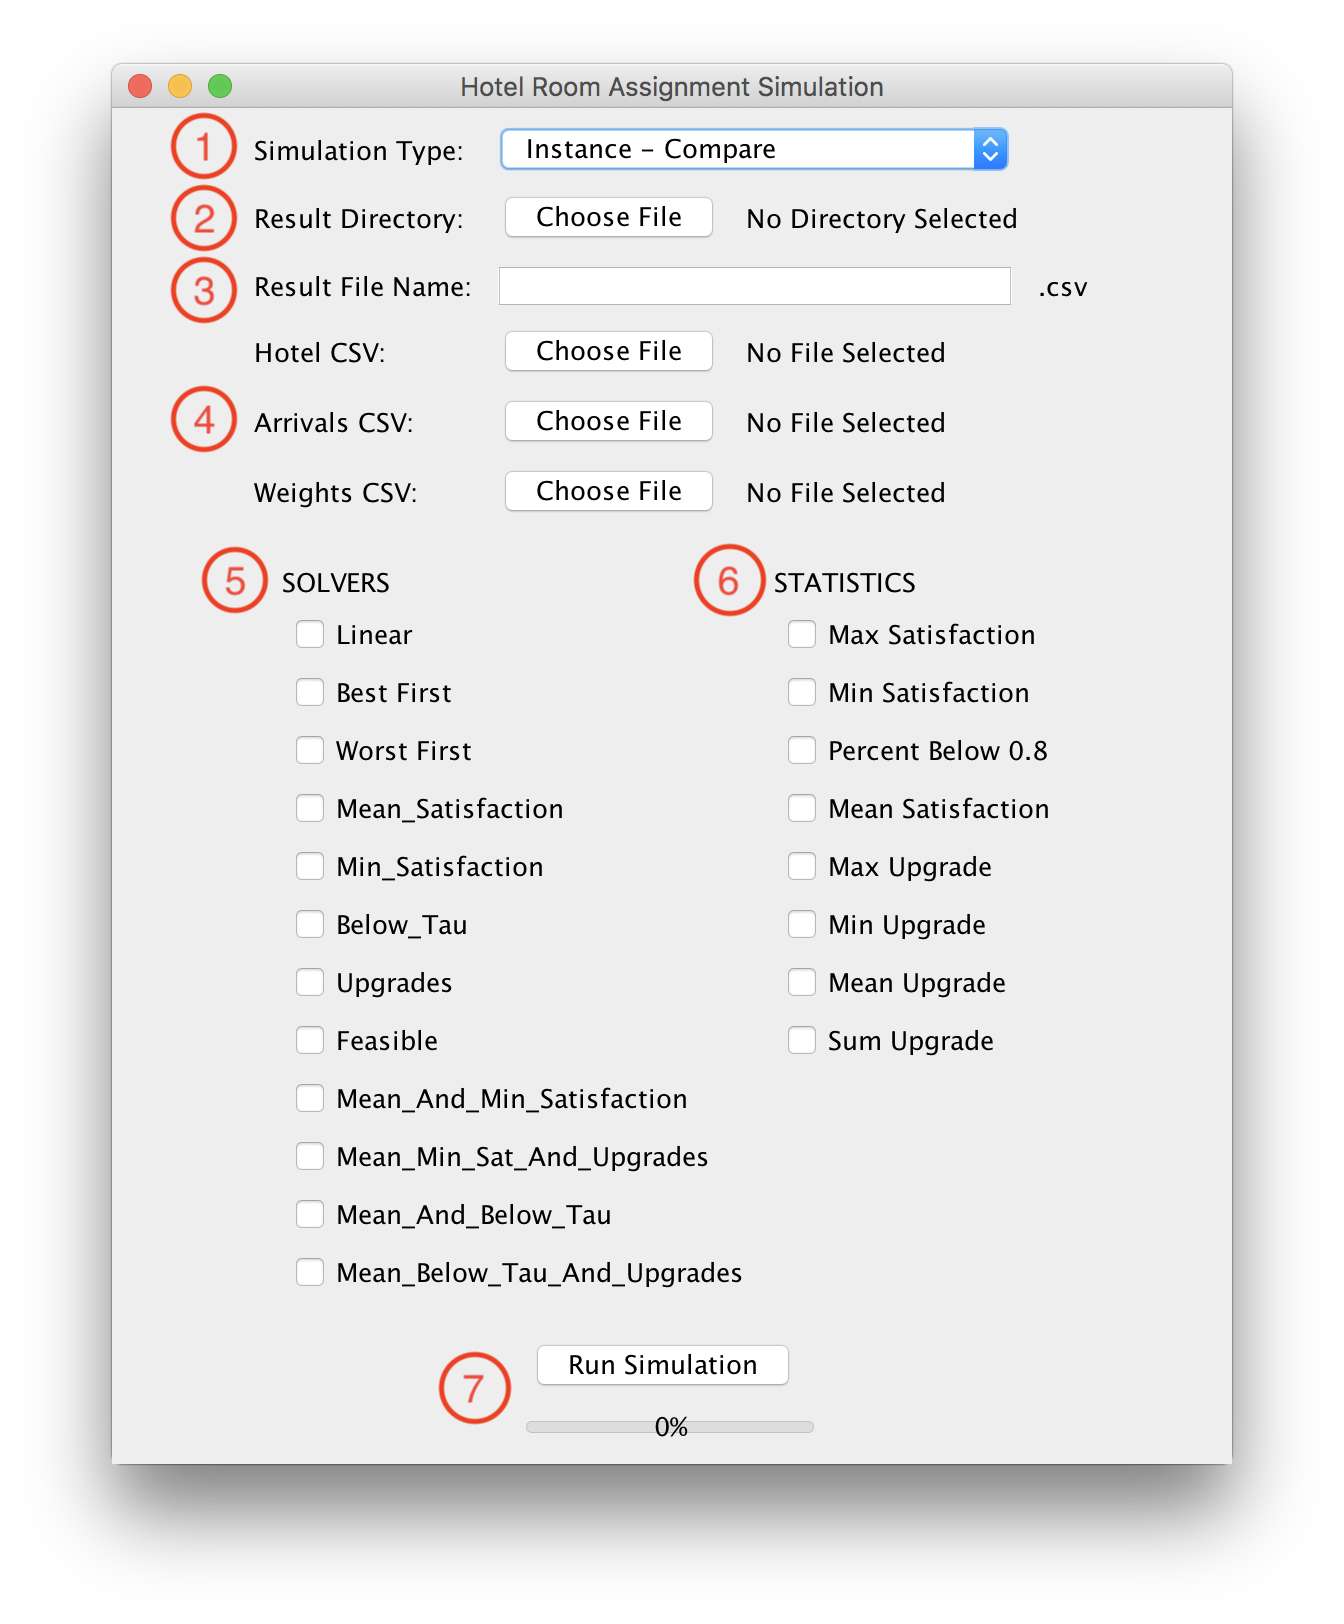
\includegraphics[scale=0.38]{images/appScreen.png}
\end{center}

\subsection{Running a Simulation}

\par Now, we walk through running a simulation on our running example. For the first simulation, we select the three heuristic solvers:
\begin{itemize}
    \item \texttt{Linear}: Assigns guests to the first available feasible room in order of arrival. Note, this heuristic is independent of guest satisfaction.
    \item \texttt{Best First}: Assigns guests to the highest quality available room in order of arrival.
     \item \texttt{Worst First}: Assigns guests to the lowest quality available room in order of arrival. This is a conservative heuristic. The idea is to maximize flexibility by leaving the highest quality rooms available. 
\end{itemize}
Additionally, we select the following statistics:
\begin{itemize}
    \item \texttt{Min Satisfaction}: Measures the satisfaction of the least satisfied guest
    \item \texttt{Mean Satisfaction}: Measures the satisfaction of the average guest
    \item \texttt{Percent Below 0.8}: Measures the percent of guests who are assigned to a room that gives them strictly less that 80\% satisfaction
    \item \texttt{Sum Upgrade}: Measures the amount of upgrading in the assignment. The upgrade an individual guest experiences is their requested type subtracted from their assigned room type. E.g. a guest requesting type 1 who is assigned type 3 has an upgrade of 2. \texttt{Sum Upgrade} measures the sum of these upgrades across all guests.
\end{itemize}
Below, we show the simulation window set for the described simulation.
\begin{center}
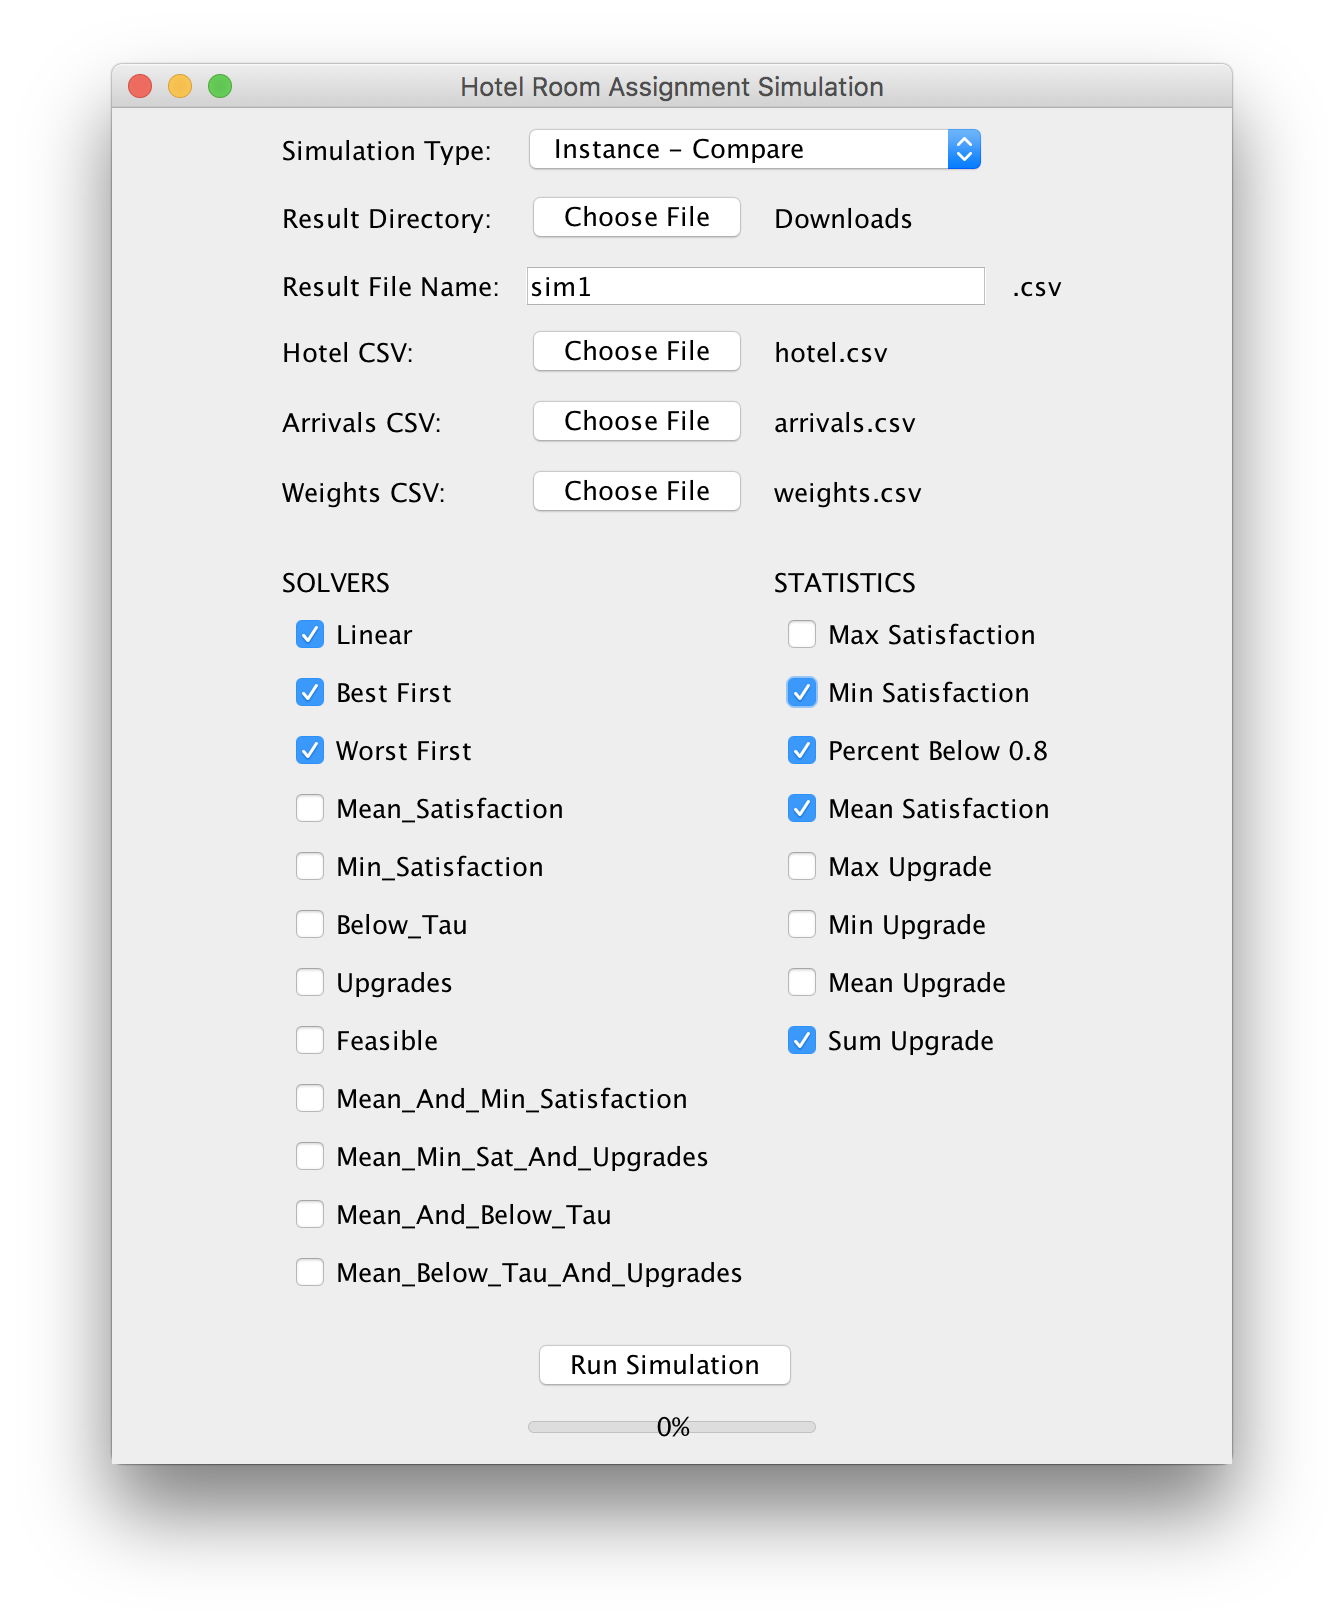
\includegraphics[scale=0.4]{images/sim1Screen.png}
\end{center}
\subsection{Interpreting the Results}
After running the above simulation, there is now a CSV file called \texttt{sim1.csv} located in the \texttt{Downloads} folder. The resulting CSV file should look like this:
\begin{figure}[H]
    \begin{center}
  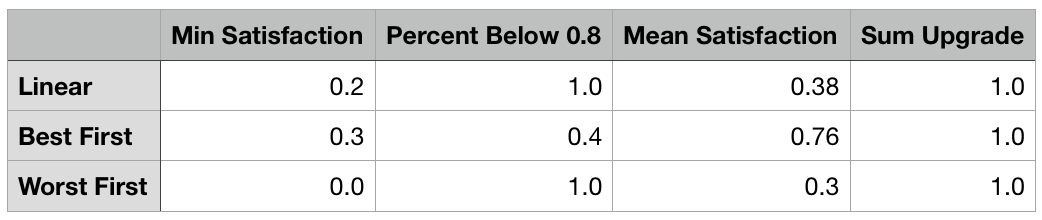
\includegraphics[scale=0.6]{images/sim1CSV.png}
  \caption{Simulation 4.3(a).}
  \end{center}
\end{figure}
\vspace{-0.5cm}
\par We can now analyze the performance of these three heuristics on our sample instance. Each row corresponds to a selected solver while each column corresponds to a selected statistic. \texttt{Best First} did significantly better than the other two heuristics with an average satisfaction of 76\% compared to 38\% and 30\%. Furthermore, only 40\% of guests had less than 80\% satisfaction in the \texttt{Best First} assignment whereas the other two heuristics saw 100\% of guests having less than 80\% satisfaction. This demonstrates some of the types of analysis that can be done with our tool. Furthermore, it highlights how variable these heuristics can be. Now, we run the simulation again after introducing a handful of optimal solvers:
\begin{itemize}
    \item \texttt{Mean\_Satisfaction}: Maximizes the mean guest satisfaction 
    \item \texttt{Min\_Satisfaction}: Maximizes the satisfaction of the least satisfied guest 
    \item \texttt{Below\_Tau}: Minimizes the number of guests that are less than 80\% satisfied with their room
    \item \texttt{Upgrades}: Minimizes the amount of upgrading in the room assignment
\end{itemize}
After running the simulation again, we have the following results.
\begin{figure}[H]
    \begin{center}
  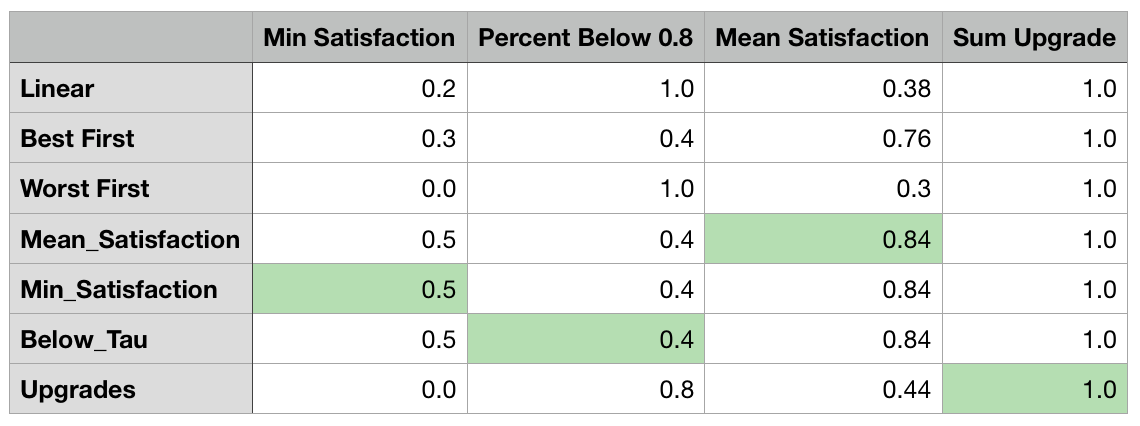
\includegraphics[scale=0.6]{images/sim2CSV.png}
  \caption{Simulation 4.3(b).}
  \end{center}
\end{figure}
\vspace{-0.5cm}
\par The cells highlighted green correspond to the optimal values for each of the statistics. We see the optimal mean and minimum satisfaction were 84\% and 50\% respectively. Note that none of the heuristics were optimal in terms of mean or minimum satisfaction. The optimal percent of guests with less than 80\% satisfaction was 40\%, which the \texttt{Best First} heuristic actually achieved. 
\par We have now walked through how to create CSV files representing an instance, specify and run a simulation, and interpret the results. However, this is far from the full functionality this tool provides. In the next sections, we walk through two more types of simulations that can be run with no programming required.
\subsection{Simulating Random Arrivals}
\par Before, we ran solvers on a specific instance. We now introduce the simulation type \texttt{Random Instance - Compare}. This type of simulation generates random (feasible) sets of arrivals for a given hotel. We can now compare solvers' performances on a specified number of random instances for a given hotel. After selecting \texttt{Random Instance - Compare} from the drop down menu, the editable fields appearing on the window will change. Now, instead of selecting an arrivals and weights CSV, we must select a ``Parameter File" and choose the number of trials or random instances to generate. The parameter file consists of adjustable parameters that describe how random instances are generated. One can adjust these to better fit their needs or default values can be used. More information on the parameters file is given in the Appendix. Here, we use the provided \texttt{demo.properties} file. Additionally, we use \texttt{hotel.csv} as the hotel CSV file and run 100 trials. The simulation window should look something like this (excluding the selected solvers and statistics).
\begin{center}
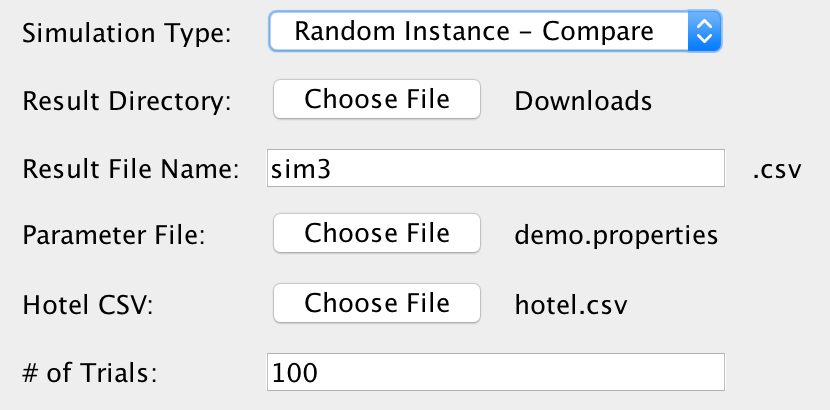
\includegraphics[scale=0.55]{images/sim3Screen.png}
\end{center}
The resulting CSV for this simulation is shown below.
\begin{figure}[H]
    \begin{center}
  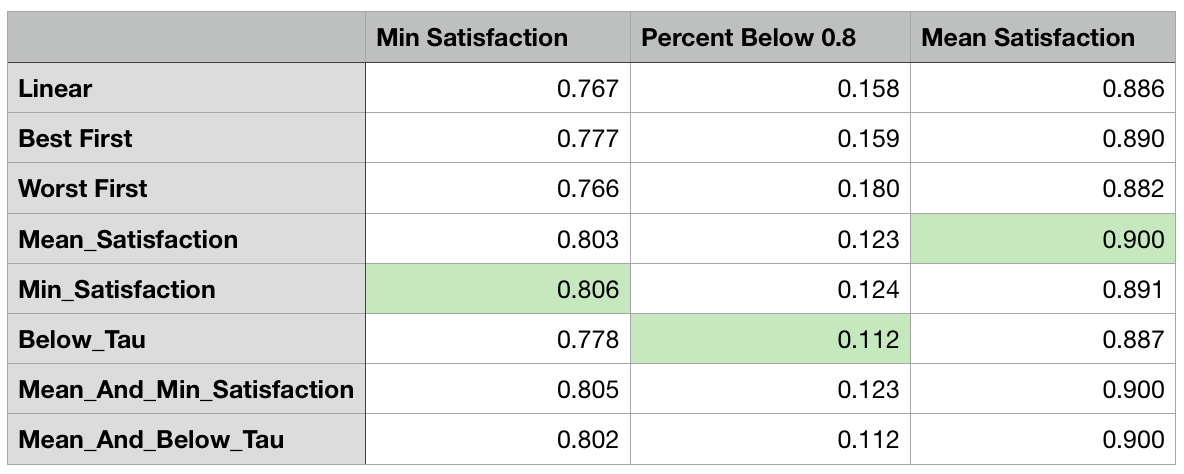
\includegraphics[scale=0.55]{images/sim3CSV.png}
  \caption{Simulation 4.4.}
  \end{center}
\end{figure}
\vspace{-0.5cm}
\par The number in each cell represents the average value over the 100 trials that were simulated. Again, the optimal values for each statistic are highlighted in green. Here, the three heuristics provided near optimal minimum and mean satisfaction. However, the percent of guests with satisfactions below 80\% was not optimal. In the case of the \texttt{Worst First} heuristic, 18\% of guests had less than 80\% satisfaction while an optimal assignment had only 11.2\%. Additionally, the solver \texttt{Mean\_And\_Below\_Tau} (which attempts to maximize mean satisfaction and minimize the percent of guests with less than 80\% satisfaction) was able to achieve optimal \texttt{Percent Below 0.8} and \texttt{Mean Satisfaction} and near optimal \texttt{Min Satisfaction} simultaneously.
\subsection{Simulating Random Instances}
\par We now introduce one last simulation that can be run without programming. A comprehensive list of simulations can be found in the Appendix. Previously, we executed solvers on specific instances and instances that were randomly generated for specific hotels. Now, we will run a simulation where instances are completely randomly generated. Again, the random generation of these instances is based on the parameters provided in the parameters file. Aside from the parameters file, the only parameter a user must provide is the number of available rooms. The distribution and number of room types will depend on the chosen (or default) parameters. The name of this simulation is \texttt{Random - Compare}. Below, we have an example simulation and the resulting CSV file. Notice the additional field Hotel Size(s). Here, one can specify the number of available rooms. Multiple sizes can be tested by listing hotel sizes separated by commas. In the below simulation, 25 trials are run on each of hotel sizes 5, 10 and 15.
\begin{center}
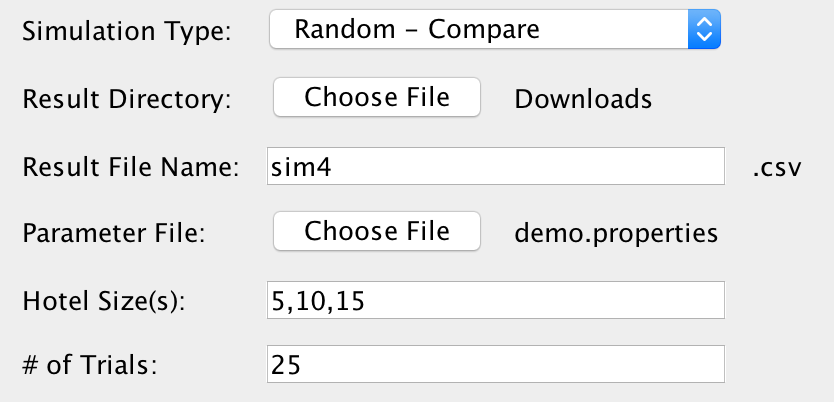
\includegraphics[scale=0.55]{images/sim4Screen.png}
\end{center}
\begin{figure}[H]
    \begin{center}
  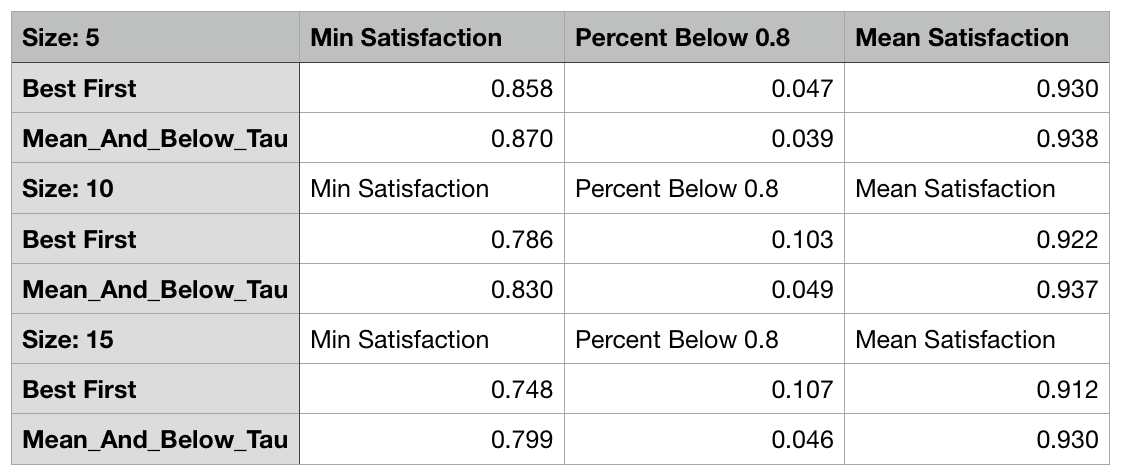
\includegraphics[scale=0.6]{images/sim4CSV.png}
  \caption{Simulation 4.5}
  \end{center}
\end{figure}
\vspace{-0.5cm}
\par The resulting CSV file consists of 3 tables, each corresponding to a tested hotel size. Each table is organized similar to previous simulations. For example, of the 25 trials run on a hotel of size 5, the mean satisfaction achieved by the \texttt{Best First} solver was 93\%. However, of the 25 trials run on a hotel of size 15, the mean satisfaction achieved by the \texttt{Best First} solver was 91.2\%. Overall, this simulation type is useful for comparing solvers in general on hotels of varying size.
\section{Programming Walk-through}
This walk-through assumes some knowledge of Java including working with Java libraries. Here, we cover how to create instances both from CSVs and randomly, run solvers, and run the simulations described in Section 4 programmatically. Additionally, we describe how to adjust parameters on solvers to yield different desired effects. We will use the same running example instance.
\subsection{Basics}
\par The first step in running a solver on a specific instance is loading the corresponding CSV files. The following lines of code demonstrate how this can be done.
\begin{center}
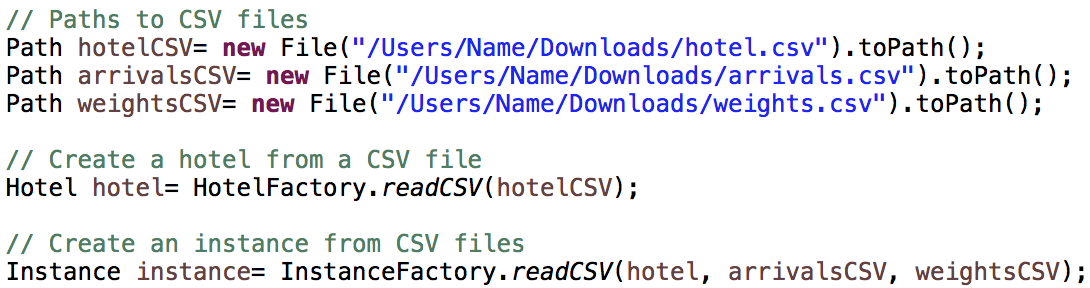
\includegraphics[scale=0.7]{images/readCSVCode.png}
\end{center}
\par To view an instance, one can use \texttt{System.out.println(instance)}. The class \texttt{Instance} represents an instance; it maintains information related to the hotel, arrivals, and guest satisfaction. The \texttt{Solver} interface takes an \texttt{Instance} and returns some \texttt{Decision}. One type of \texttt{Decision} is an \texttt{Assignment} which represents an assignment of guests to rooms for some instance. Furthermore, an \texttt{Assignment} maintains statistics related to an assignment such as mean guest satisfaction. Every room assignment solver implements \texttt{Solver<Assignment>}. Thus, it takes an \texttt{Instance} and returns an \texttt{Assignment} for that instance. The next lines of code create a handful of solvers and show how to use them to produce a room assignment.
\begin{center}
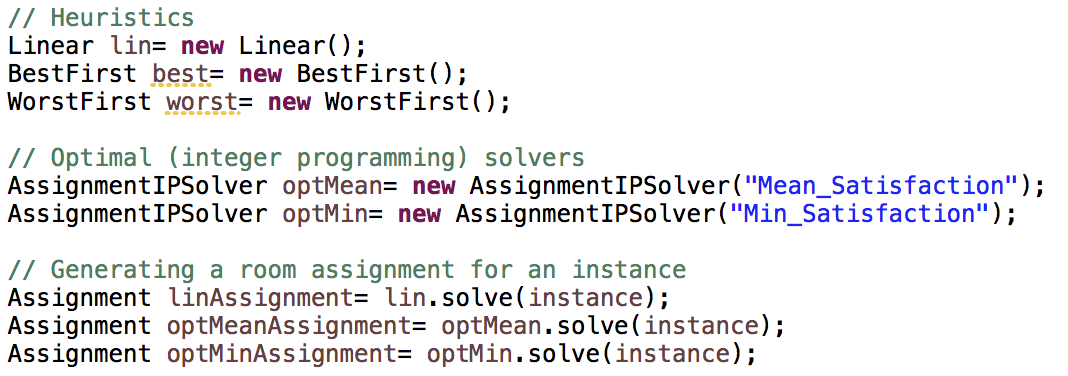
\includegraphics[scale=0.7]{images/runSolversCode.png}
\end{center}
\par Similarly, to view an assignment, one can use \texttt{System.out.println(assignment)}. In addition to viewing the assignment itself, we can also use this tool to get certain statistics about that assignment. The \texttt{Statistic} interface takes a \texttt{Decision} such as an \texttt{Assignment} and returns a \texttt{Double} corresponding to the value of that statistic for the given \texttt{Decision}. Any statistic for a room assignment implements \texttt{Statistic<Assignment>}. It takes an \texttt{Assignment} and returns the value of the statistic. Below, we create a handful of statistics and evaluate the room assignments from before.
\begin{center}
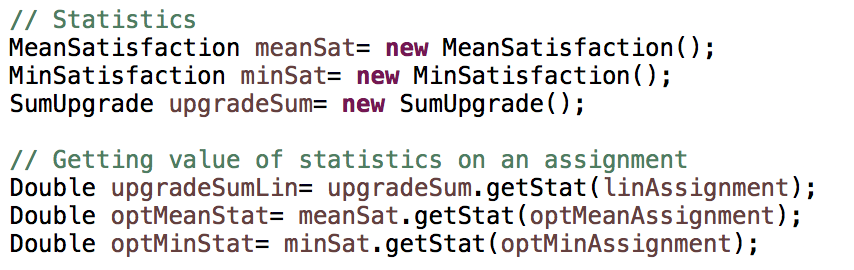
\includegraphics[scale=0.7]{images/runStatsCode.png}
\end{center}
\par This covers the basics of creating an instance, running a solver, and evaluating the room assignment. Simulations can also be run programmatically. A \texttt{Simulation} is a \texttt{Thread} which takes some simulation parameters, runs the simulation, and then writes the results of the simulation to a CSV file. The code to run Simulation 4.3(a) from Section 4 is shown below as an example.
\begin{center}
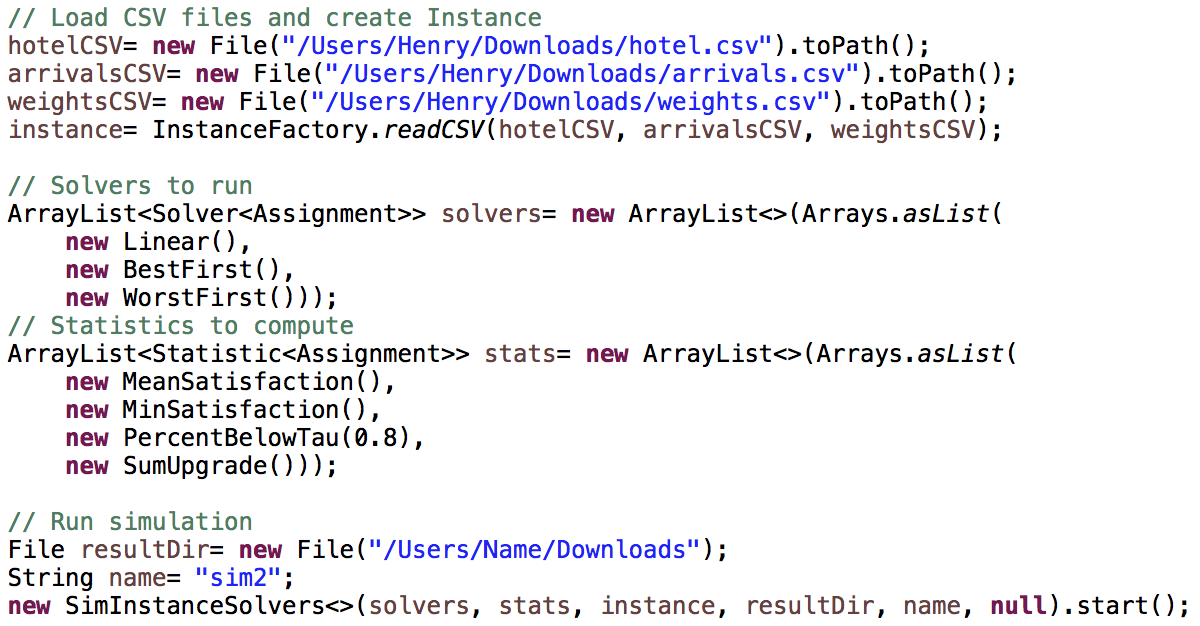
\includegraphics[scale=0.6]{images/runSimCode.png}
\end{center}
\subsection{Solver Parameters}
\par The Graphical User Interface (GUI) in Section 4 uses some solvers that can take additional parameters. These solvers are set to default values for the GUI. However, when running solvers programmatically, these parameters can be specified explicitly. One type of room assignment solver is \texttt{AssignmentIPSolver}. This solver utilizes AMPL and integer linear programming to achieve optimal room assignments. However, optimal is a vague term. We must specify exactly what we wish to optimize. Do we want to maximize the mean satisfaction of a guest? Do we want to minimize the number of upgrades given? The value we wish to maximize or minimize is commonly referred to as an objective function in integer linear programming. The \texttt{AssignmentIPSolver} takes a \texttt{String} representing the name of the objective function. For example \texttt{Mean\_Satisfaction} is the objective function which maximizes mean guest satisfaction. Hence, \texttt{new AssignmentIPSolver("Mean\_Satisfaction")} creates a solver producing room assignments maximizing mean guest satisfaction.
\par This raises the question: what if we want to optimize multiple different objective functions? One way to handle this is to use a weighted objective function. Here, multiple different objectives are weighted in a single objective function. For example, the weighted objective function \texttt{Mean\_Min\_Sat\_And\_Upgrades} consists of the objectives \texttt{Mean\_Satisfaction}, \texttt{Min\_Satisfaction}, and \texttt{Upgrades} weighted by $\alpha$, $\beta$, and $\gamma$ respectively:
$$\text{max} \quad \alpha(\texttt{Mean\_Satisfaction}) + \beta(\texttt{Min\_Satisfaction}) - \gamma(\texttt{Upgrades}).$$
The default values (for this weighted objective function and all others) are $\alpha = \beta = \gamma = 1$. This is \textit{approximately} equivalent to saying we care about each of these objectives equally. That is, we want to maximize both measures of satisfaction just as much as we want to minimize upgrades. The nice thing about weighted objective functions is the weights can be tweaked if we do not get the desired results. For example, say we run \texttt{Mean\_Min\_Sat\_And\_Upgrades} with default weights. In the resulting room assignment, the guests are very satisfied. However, many are upgraded to higher room types. While we want satisfied guests, we can't afford to upgrade everyone. We can adjust the weights to reflect this. Say we value the \texttt{Upgrades} objective twice as much as the \texttt{Mean\_Satisfaction} and \texttt{Min\_Satisfaction} objectives. To achieve this, we set $\alpha =\beta = 1$ and $\gamma = 2$.
\begin{center}
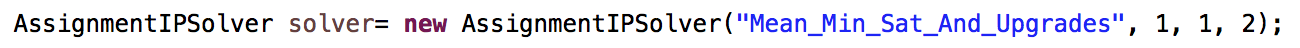
\includegraphics[scale=0.7]{images/weightedObj.png}
\end{center}
\par There is another solver which takes additional parameters although it is not a weighted objective function. This solver is \texttt{Below\_Tau}. It minimizes the number of guests with a satisfaction less than some threshold $\tau$. In Section 4, we set this to the chosen default value of $\tau = 0.80$. However, we can set this threshold to any satisfaction between 0\% and 100\%. The following code will create a solver that minimizes the number of guests with a satisfaction less than $\tau =$ 90\%.
\begin{center}
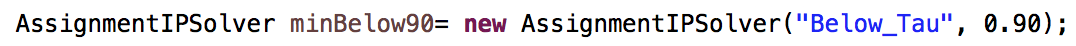
\includegraphics[scale=0.7]{images/BelowTauCode.png}
\end{center}
\par As a final exercise, we examine the performance of a handful of \texttt{Below\_Tau} solvers with varying values for $\tau$. We provide an outline of the code below. First, we create three \texttt{Below\_Tau} solvers with $\tau$ set to 0.80, 0.85, and 0.90. Next, we generate a random instance on a hotel of size 25 and solve this instance using each solver. To analyze the solver's preformance, we construct a room assignment statistic called \texttt{PercentBelowTau}. Given a room assignment, \texttt{PercentBelowTau} returns the number of guests in the assignment with satisfaction less that $\tau$ where $\tau$ is a parameter of the statistic. Here, we set $\tau = 0.90$. Lastly, we get the value of this statistic for every assignment and print the results. 
\begin{center}
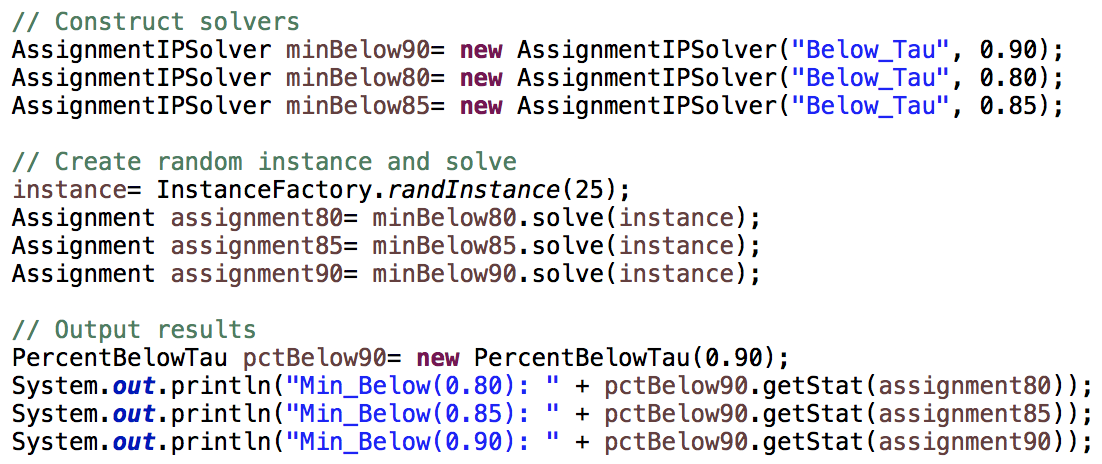
\includegraphics[scale=0.7]{images/BelowTauEx.png}
\end{center}

The console output is shown below. The solver minimizing the number of guests below 90\% satisfaction resulted in only 15\% (compared to 30\% and 35\%) of guests having a satisfaction below 90\%. By raising the value of $\tau$ for the solver, we achieve an arguably better assignment with 85\% of guests having a satisfaction greater than 90\%. 
\begin{center}
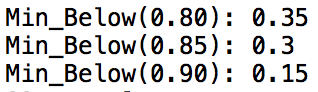
\includegraphics[scale=0.7]{images/results.png}
\end{center}
\par This concludes the walk-through. We have shown how to replicate the simulations done in the non-programming walk through. Furthermore, we have presented how solver and statistic parameters can be set explicitly to achieve a wider range of functionality than available in the GUI. A comprehensive list of solvers, statistics, and their parameters is given in the Appendix.

\newpage

\appendix
\section{Appendix}


\subsection{List of Simulations}

\par The following is a comprehensive list of currently implemented simulations related to room assignments for hotels. 

\begin{center}
\begin{tabular}{|l|p{12cm}|}
\hline
\textbf{Simulation Name} & \textbf{Description} \\
\hline
\texttt{SimAddGuest} & For some set of hotel sizes, a specified number of instances are randomly generated. Then, the average mean satisfaction across all trials for each hotel size is recorded before and after an additional guest is accommodated. This simulation allows one to asses the risk of accepting an additional reservation under various conditions. \\
\hline
\texttt{SimHotel} & For a specific hotel, a specified number of instances are randomly generated. Then, a given set of solvers are executed on every random instance and a given set of statistics are recorded. The average value of every statistic for every solver is returned. This allows for the comparison of solvers on a specific hotel in the long run.  \\
\hline
\texttt{SimInstanceSolvers} & For a specific hotel, a given set of solvers are executed and a given set of statistics are recorded. This allows for the comparison of solvers on a specific instance.  \\
\hline
\texttt{SimParameters} & A weighted objective function is chosen. A set of weights are given for $\alpha$, $\beta$, and $\gamma$ respectively. A set of solvers is then constructed using every possible combination of the given weights. The simulation then generates a specified number of random instances of a given size. Each solver is executed on every instance and a given set of statistics are recorded. The average value of every statistic across all random instances is then recorded for every combination of the given weights. Using this simulation, one can identify the best weights to choose for a solver utilizing a weighted objective function.    \\
\hline
\texttt{SimRunTimes} &  For some set of hotel sizes, a specified number of instances are randomly generated. Then, some set of solvers are run on every instance and the run time is recorded. The average run time for every solver on every hotel size is then returned. \\ 
\hline
\texttt{SimShowTrials} & A specified number of instances of a given size are randomly generated. Then, a set of solvers are executed on every instance and a chosen statistic is recorded. The result of every random instance is returned. As opposed to simply returning averages across a number of trials, this simulation returns the results of every trial allowing one to view the distribution of a statistics for multiple solvers.   \\
\hline
\texttt{SimSolvers} & For some set of hotel sizes, a specified number of instances are randomly generated. Then, a given set of solvers are executed on every random instance and a given set of statistics are recorded. For all hotel sizes, the average value of every statistic for every solver is returned. This allows for a general comparison of solvers at different hotel sizes \\
\hline
\end{tabular}
\end{center}

\newpage

\subsection{List of Solvers and Statistics}

\par Below, are the current solvers and statistics related to room assignment.

\begin{center}
\textbf{Solvers} 
\end{center}
\begin{center}
\begin{tabular}{|l|p{4.4cm}|l|}
\hline
\textbf{Solver Name} & \textbf{Description} & \textbf{Parameters} \\
\hline
\texttt{Mean\_Satisfaction} & Maximizes the mean guest satisfaction &  \\
\hline
\texttt{Min\_Satisfaction} & Maximizes the minimum guest satisfaction &  \\
\hline
\texttt{Below\_Tau} & Minimizes the number of guests who have a satisfaction less than $\tau$ & $\tau$: satisfaction threshold  \\
\hline
\texttt{Upgrades} & Minimizes the amount of upgrading. Specifically, minimizes the statistic \texttt{SumUpgrade} & \\
\hline
\texttt{Guest\_Satisfaction} & Maximizes a given guests satisfaction & \texttt{guest}: hotel guest \\
\hline
\texttt{Mean\_And\_Min\_Satisfaction} & Weighted obj. func.  & $\alpha$: weight for \texttt{Mean\_Satisfaction} \\
& & $\beta:$ weight for \texttt{Min\_Satisfaction} \\
\hline
\texttt{Mean\_Min\_Sat\_And\_Upgrades} & Weighted obj. func.  & $\alpha$: weight for \texttt{Mean\_Satisfaction} \\
& & $\beta:$ weight for \texttt{Min\_Satisfaction} \\
& & $\gamma:$ weight for \texttt{Upgrades} \\
\hline
\texttt{Mean\_And\_Below\_Tau} & Weighted obj. func.  & $\tau$: satisfaction threshold \\
& & $\alpha$: weight for \texttt{Mean\_Satisfaction} \\
& & $\beta:$ weight for \texttt{Below\_Tau} \\
\hline
\texttt{Mean\_Below\_Tau\_And\_Upgrades} & Weighted obj. func.  & $\tau$: satisfaction threshold \\
& & $\alpha$: weight for \texttt{Mean\_Satisfaction} \\
& & $\beta:$ weight for \texttt{Below\_Tau} \\
& & $\gamma:$ weight for \texttt{Upgrades} \\
\hline
\end{tabular}
\end{center}

\vspace{1cm}
\begin{center}
\textbf{Statistics}
\end{center}
\begin{center}
\begin{tabular}{|l|l|l|}
\hline
\textbf{Statistic Name} & \textbf{Description} & \textbf{Parameters} \\
\hline
\texttt{MaxSatisfaction} & Satisfaction of the most satisfied guest & \\
\hline
\texttt{MinSatisfaction} & Satisfaction of the least satisfied guest & \\
\hline
\texttt{PercentBelowTau} & Percent of guests with a satisfaction below $\tau$ & $\tau$: satisfaction threshold \\
\hline
\texttt{MeanSatisfaction} & Average satisfaction of a guest & \\
\hline
\texttt{MaxUpgrade} & Largest upgrade in the assignment  & \\
\hline
\texttt{MinUpgrade} & Smallest upgrade in the assignment  & \\
\hline
\texttt{MeanUpgrade} & Average upgrade in the assignment  & \\
\hline
\texttt{SumUpgrade} & Sum of upgrades in the assignment  & \\
\hline
\end{tabular}
\end{center}

\newpage

\subsection{The Parameters File}

\par The parameters file is a \texttt{.properties} file that maintains the parameters used to randomly generate instances. The parameters in this file can be adjusted to accurately reflect what is observed in various hotel markets. The parameters file used in this walk-through is \texttt{demo.properties}. A list of parameters, their description, and their value in \texttt{demo.properties} is given below.

\begin{center}
\begin{tabular}{|l|l|c|}
\hline
\textbf{Description} & \textbf{Parameter} & \textbf{Value} \\
\hline
Minutes per time interval & \texttt{timeInterval} & 30 \\
Average hotel capacity & \texttt{avgCapacity} & 0.8 \\
Housekeepers to rooms ratio & \texttt{housekeepingRatio} & 0.10 \\
Number of room types & \texttt{roomTypes} & 3 \\
Distribution of room types & \texttt{roomDist} & $[0.7,0.15,0.15]$ \\
(Eg. 15\% of rooms are type 3) & & \\
Distribution of room type requests & \texttt{requestDist} & $[0.7,0.15,0.15]$ \\
(Eg. 70\% of requests are for rooms type 1) & & \\
Normal distribution for room clean time (by type)& \texttt{cleanTimeMean} & $[30,60,60]$ \\
& \texttt{cleanTimeStd} & $[5,10,10]$ \\
Lower and upper bound of room clean times (by type) & \texttt{cleanTimeLb} &  $[30,30,30]$ \\
& \texttt{cleanTimeUb} & $[60,90,90]$ \\
Normal distribution for room quality & \texttt{qualityMean} & 0.8 \\
& \texttt{qualityStd} & 0.2 \\
Beta distribution for upper bound of guest satisfaction & \texttt{ubBetaA} & 10 \\
& \texttt{ubBetaB} & 0.5 \\
Beta distribution for lower bound of guest satisfaction & \texttt{lbBetaA} & 2.5 \\
& \texttt{lbBetaB} & 0.5 \\
Adds additional randomness to guest satisfaction & \texttt{randSat} & 0.001 \\
($S_{ij} = L_i + (U_i - L_i)V_j + N(0,\texttt{randSat}))$& & \\
Satisfaction bonus if upgraded & \texttt{upgradeBonus} &  0 \\
Normal distribution for guest checkout times & \texttt{checkoutMean} & 660 \\
& \texttt{checkoutStd} & 30 \\
Lower and upper bound for guest checkout times & \texttt{checkoutLb} & 360 \\
& \texttt{checkoutUb} &  780 \\
Normal distribution of guest check in times & \texttt{checkinMean} & 900 \\
& \texttt{checkinStd} & 30 \\
The lower and upper bound of guest check out times & \texttt{checkinLb} & 840 \\
& \texttt{checkinUb} & 1200 \\
\hline
\end{tabular}
\end{center}

NOTE: All times are given in minutes. E.g. average checkout time is 660 minutes or 11AM.

\end{document}
